%%%%%%%%%%%%%%%%%%%%%%%%%%%%%%%%%%%%%%%%%%%%%%%%%%%%%%%%%%%%%%%%%%%%%%%%%%%%%%%%
%2345678901234567890123456789012345678901234567890123456789012345678901234567890
%        1         2         3         4         5         6         7         8

\documentclass[letterpaper, 10 pt, conference]{ieeeconf}  % Comment this line out if you need a4paper

%\documentclass[a4paper, 10pt, conference]{ieeeconf}      % Use this line for a4 paper

\IEEEoverridecommandlockouts                              % This command is only needed if 
                                                          % you want to use the \thanks command

\overrideIEEEmargins     


 

    

% Needed to meet printer requirements.
\usepackage{graphicx}

%In case you encounter the following error:
%Error 1010 The PDF file may be corrupt (unable to open PDF file) OR
%Error 1000 An error occurred while parsing a contents stream. Unable to analyze the PDF file.
%This is a known problem with pdfLaTeX conversion filter. The file cannot be opened with acrobat reader
%Please use one of the alternatives below to circumvent this error by uncommenting one or the other
%\pdfobjcompresslevel=0
%\pdfminorversion=4

% See the \addtolength command later in the file to balance the column lengths
% on the last page of the document

% The following packages can be found on http:\\www.ctan.org
%\usepackage{graphics} % for pdf, bitmapped graphics files
%\usepackage{epsfig} % for postscript graphics files
%\usepackage{mathptmx} % assumes new font selection scheme installed
%\usepackage{times} % assumes new font selection scheme installed
%\usepackage{amsmath} % assumes amsmath package installed
%\usepackage{amssymb}  % assumes amsmath package installed

\title{\LARGE \bf
Designing Social Robots for Mental Heath Care
}
%Social Robots for Early Detection of Mental Heath Conditions
\author{Amrita Krishnaraj$^{1}$ and Chien-Ming Huang$^{2}$% <-this % stops a space
\thanks{$^{1}$Amrita Krishnaraj is with the Laboratory for Computational sensing and Robotics,
        Johns Hopkins University, Baltimore, MD 21218, USA.
        {\tt\small akrishn9@jhu.edu}}%
\thanks{$^{2}$ Chien-Ming Huang is with the Department of Computer Science, Johns Hopkins University, Baltimore, MD 21218, USA.
        {\tt\small cmhuang@cs.jhu.edu}}%
}



\begin{document}



\maketitle
\thispagestyle{empty}
\pagestyle{empty}


%%%%%%%%%%%%%%%%%%%%%%%%%%%%%%%%%%%%%%%%%%%%%%%%%%%%%%%%%%%%%%%%%%%%%%%%%%%%%%%%
\begin{abstract}
Mental health is a growing socio-economic burden worldwide and leads to negative ramifications including mortality and poor quality of life. Successful prevention, detection, and intervention of mental illness will make a significant, positive economic and societal impact. This research broadly explores how social robots may contribute to effective mental health care. In this work, we present our initial effort in designing and developing  a social robot that detects emotional states through multimodal sensing of human behavior and provides affective companionship. We describe a pilot study exploring how people might interact with and perceive the robot. Our preliminary results show that participants treated the robot socially and engaged in affective interactions with the robot. 
\end{abstract}


%%%%%%%%%%%%%%%%%%%%%%%%%%%%%%%%%%%%%%%%%%%%%%%%%%%%%%%%%%%%%%%%%%%%%%%%%%%%%%%%
\section{INTRODUCTION}
Mental health is a growing concern globally. Around 1-in-6 people in the world experience one or more mental illnesses \cite{r1}. The financial burden associated with mental illness is substantial and costs America approximately \$193.2 billion per year \cite{r3}. Individuals living with mental illness face an increased risk of chronic medical conditions, increased risk of suicide, and involvement in anti-social activities. Despite being critical to overall well-being and physical health, diagnoses and treatment of mental illnesses remain low. Emerging research indicates that intervening early can interrupt the negative course of some mental illnesses and may, in some cases, lessen long-term disability \cite{r2}. 

As evidenced by successful applications in care for individuals with autism (e.g., \cite{scassellati2018improving}), Socially Assistive Robots (SARs) \cite{S1} represents a promising tool for mental health care. While prior research has explored how SARs might provide social, emotional support and companionship (e.g., \cite{p1}), this work investigates how a social robot may be used for early detection of mental health conditions. In particular, we leverage the embodiment and tangibility of a social robot and seek to infer a person's psychological states through multimodal sensing of human behavior, including auditory, visual, and haptic cues. 
Affective touch is a crucial element of social bonding and for affective communication and provides rich information for understanding a person's emotional state. We envision that such a social robot will help identify the unobserved psychological stressors to better inform therapy.

\begin{figure}[t!]
\centering

\includegraphics[width=3.4in]{teaser.pdf}
\vskip -10pt
\caption{Left: Our social robot is designed to afford affective interactions through touch, hug, and other haptic gestures. Right: Our prototype robot responds socially through nonverbal behaviors based on detected human interaction behaviors.}
\label{fig:teaser}
\end{figure}

\section{ROBOT DESIGN}
The physical dimensions of the robot are 17x15x30 centimeters and weighs about 2.36 lbs. The robot has 6 DOF, eye-lids open and closing mechanism (2 DOF), eyeballs pan and tilt mechanism (2 DOF), and neck rotation mechanism (2 DOF). The entire robot is covered with artificial fur to encourage the users to make physical contact with the robot. It is equipped with a camera, a microphone, an IMU, and tactile sensors.  

\begin{figure*}[t!]
\centering
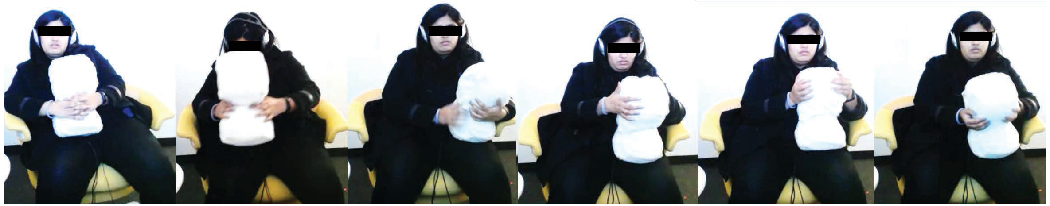
\includegraphics[width=\textwidth]{pilot-data.pdf}
\vskip -10pt
\caption{Interaction examples from our pilot study. The participant engaged with the robot through various forms of affective touch.}
\label{fig:pilot-study}
\end{figure*}

The robot consists of several software modules that sense, interpret, and respond to human behaviors. The gesture recognition module makes use of the contact information obtained from the tactile sensors that cover the robot to classify the haptic contact into a gesture. The gestures that the robot can recognize include stroke, contact, hug, hold, rub, pat, and squeeze. In addition, the IMU data is analyzed to infer the robot's posture such as toss, rock, and lift.  

The face tracking module utilizes the Single Short MultiBox detector (SSD) for face detection and seeks to maintain the detected face at the centre of robot's visual field. The emotion recognition module takes the sensor (camera, microphone, and tactile) inputs and interprets the emotional state of the user. In particular, visual emotion is recognized using the mini-Xception network, while auditory emotion is obtained from a train DNN network. The details of the design of the robot are documented in \cite{r4}. 

The robot is designed to respond nonverbally to human interactions. Its nonverbal responses are generated through two layers: a behavior-planning layer and a behavior generation layer. The robot's behavior is based on its internal states, which is influenced by the user's inferred emotions. The behavior-planning layer takes input from the modules of face tracking and emotion detections to determine the robot's internal state. This layer then decides a particular response from a pool of predefined responses and sends basic behavioral patterns to the behavior-generation layer. The behavior-generation layer generates control references for each actuator in order to perform the behavior coherently. The behavior-generation layer adjusts the priority of behaviors based on the robot's internal states. This design creates lifelike behavior for affective interactions.

%\subsection{Haptic and Posture Cues}

%A fabric tactile sensor, formed by sandwiching a resistive fabric between two conductive fabrics resulting in a matrix of $mxn$ contact points, is used for obtaining tactile information. Due to contact, the pressure increases and the pressure at each point is derived by measuring the potential difference across it. The contact regions in addition to previous contact history is used to classify the tactile input into one of the haptic gestures.  is achieved using the 6 DOF IMU. posture analysis is performed from the data received from the IMU to inform the robot about its surrounding and its position relative to the user.

%based on \cite{} is used for real-time detecting of faces. This detector is trained on both FER2013 \cite{} and IMDB \cite{} data sets and achieves an accuracy of 93\% in general object detection task together with real-time run-time performance (59FPS). In order to track the person across the room, the face position is maintained at the centre of the camera image plane. The difference is face position between successive images is considered as error and linear rotation is performed to maintain the face at the center of image using the control law.  Only the translation along the x and z axis is considered, a linear rotation at the neck is made to minimize the error vector.

%\subsection{Emotion Classification Framework}

%Emotion recognition module: 
%First, the audio signal is segmented and then the trained DNN network computes the emotion state distribution for each segment. The frames of video obtained from the camera is fed through the mini-Xception network to obtain the confusion matrix. The mini-Xception network is trained on FER-2013 data set and achieves 82.6\% accuracy. In order to synchronize the audio and video frames, a time stamp is attached to each video frame and audio segment and the average emotion of all the frames corresponding to an audio segment is used for prediction of emotion. Finally the two probabilities are combined using the Hidden Markov Model to obtain an emotional state with an accuracy of 92.3\%. 

\section{A PILOT EXPERIMENT}
We conducted a pilot, exploratory study to explore how people might interact and perceive our designed robot. Two female participants were involved in this study. During the study, artificial emotions including anger, neutral, happy, fear, amusement, and sadness were simulated and the interaction between the robot and user under different emotions was observed. 
The emotions were stimulated by viewing a video for 22 minutes which was created using the Ravdness and International Affect Picture System datasets \cite{d1}. 
%After the task, a questionnaire was administered to the subject followed by a short interview. In addition, the entire experiment was recorded for analysis. 

%To study the effectiveness of the robot, two participants, both female (M=23 yrs) who had not previously interacted with DOT were recruited from the local campus community through convenience sampling. The study took place in a controlled lab environment which was set like a home-theatre with a comfortable chair and side table.  
%The subjects were first introduced to DOT. The experimenter pointed out some of the capabilities of the robot(such as emotion recognition and face tracking) and indicated a list of haptic cues that the robot can interpret. During the study, artificial emotions were simulated in the participants. This was achieved by the participant watching a video for 22 mins which was created using the ravdness \cite{} and International Affect Picture System \cite{} data-sets. The different emotions triggered were happiness, fear, sadness, anger, amusement, disgust and calmness. The participants were allowed to interact with the robot without any restrictions.  

%\subsection{Measures}
%The questionnaire covered several topics including the interactions between the subject and robot; and DOT’s actions and expressions. In order to objectively investigate the interaction of the participants with DOT, the activities of the participants during the study was recorded.

\subsection{Preliminary Results}
The participants were excited to meet the robot and greeted it friendly during the introduction.
We observed that the participants interacted with the robot willingly from the beginning and throughout the session. They spoke to it, and stroked and hugged it. During the study, the participants held the robot on their lap when watching the video and patted it from time to time. We observed that participants held the robot facing outward to the presented video stimuli for most parts of the experiment. However, the participants turned the robot to face themselves at points when they wanted to talk to the robot or were ``checking on'' the robot as if they were making sure the robot was not having a dramatic experience. Fig. \ref{fig:pilot-study} shows some sample interactions between a participant and the prototype robot. 

\section{FUTURE WORK AND CONCLUSION} %CMH: from here:
In this work, we explore the use of social robots for early detection of mental illnesses and provide artificial emotional support. 

To this effect, a social robot was designed and a haptic, visual and audio based emotion recognition, and reactive responses were implemented. Further, in investigating how to provide artificial emotional support, a proactive nonverbal behavior set has been developed and experimented though a pilot study. This work informs future research on the design of robots and motivates the integration of social robots for early detection of mental illnesses. 

In the future, we aim to conduct field deployment of robots in hospitals and individual homes to understand how people with mental conditions live in their natural environments and how robots might be integrated. Such inclusion of field studies will bridge the gap between controlled laboratories and real-world environments. 

\section{ACKNOWLEDGEMENT}
This work is supported by the Malone Center for Engineering in Healthcare and the Johns Hopkins University. We thank Erica Hwang for her contribution to this work.

\bibliographystyle{IEEEtran}
\bibliography{2019-dgrs}

%\begin{thebibliography}{99}
%
%\bibitem{r1} H. Ritchie and M. Roser, "Mental Health," 2019. [Online].Available: https://ourworldindata.org/mental-health. [Accessed: 15- Jun- 2019]. 
%\bibitem{r2} American Mental Health Councillors Association, "Need for Early Mental Health Screening," 2011.[Online].Available: https://www.amhca.org/HigherLogic/System/DownloadDocumentFile .ashx?DocumentFileKey=2ca60afe-8be0-af27-2ad9-7100b61ad636&forceDialog=0. [Accessed: 15- Jun- 2019]. 
%\bibitem{r3} T. Insel, "Assessing the Economic Costs of Serious Mental Illness," American Journal of Psychiatry, vol. 165, no. 6, pp.663-665,2008.
%\bibitem{r4} A. Krishnaraj, “Designing Social Robots for Early Detection of Mental Heath Conditions,” (M.S. thesis), Whiting School of Eng., Johns Hopkins Univ., Baltimore, 2019.
%\bibitem{r5} C.W. Colton and R.W. Manderscheid, "Congruencies in increased mortality rates, years of potential life lost, and causes of death among public mental health clients in eight states," Preventing chronic Diseases,vol. 3, no. 2,    Apr 2006. 
%\bibitem{sc1} Scassellati, B., Boccanfuso, L., Huang, C.M., Mademtzi, M., Qin, M., Salomons, N., Ventola, P. and Shic, F., 2018. Improving social skills in children with ASD using a long-term, in-home social robot. Science Robotics, 3(21).
%
%\bibitem{p1} Wada, K., Shibata, T., Saito, T. and Tanie, K. (2006). Robot assisted activity at a health service facility for the aged for ten weeks: An interim report of a long-term experiment. Proceedings of the Institution of Mechanical Engineers, Part I: Journal of Systems and Control Engineering, 220(8), pp.709-715.
%
%\bibitem{S1} Feil-Seifer, D.and Feil-Seifer, D. and Mataric, M.J. (2005). Defining Socially Assistive Robotics. In: 9th International Conference on Rehabilitation Robotics. Chicago: Proceedings of 2005 IEEE, pp.465-468.
%
%\bibitem{d1}  Eerola, T. and Vuoskoski, J. (2010). A comparison of the discrete and dimensional models of emotion in music. Psychology of Music, 39(1), pp.18-49.
%
%\end{thebibliography}

\end{document}
